\chapter{Tinjauan Pustaka}

\section{Satelit LAPAN-A3}

Satelit LAPAN-A3 merupakan satelit yang diluncurkan oleh LAPAN pada 22 Juni
2016 bersama satelit CartoSat-2C milik \textit{Indian Space Research
Organization} (ISRO) dari Sriharikota, India. Satelit ini adalah satelit ketiga
yang telah diluncurkan LAPAN setelah LAPAN-A1/TUBSAT dan LAPAN-A2/ORARI serta
merupakan hasil kerja sama LAPAN dengan IPB \cite{hasbi2013}. Gambar
\ref{fig:a3overview} menunjukkan desain LAPAN-A3.

\begin{figure}[!ht]
\setlength\belowcaptionskip{-0.7\baselineskip}
\begin{center}
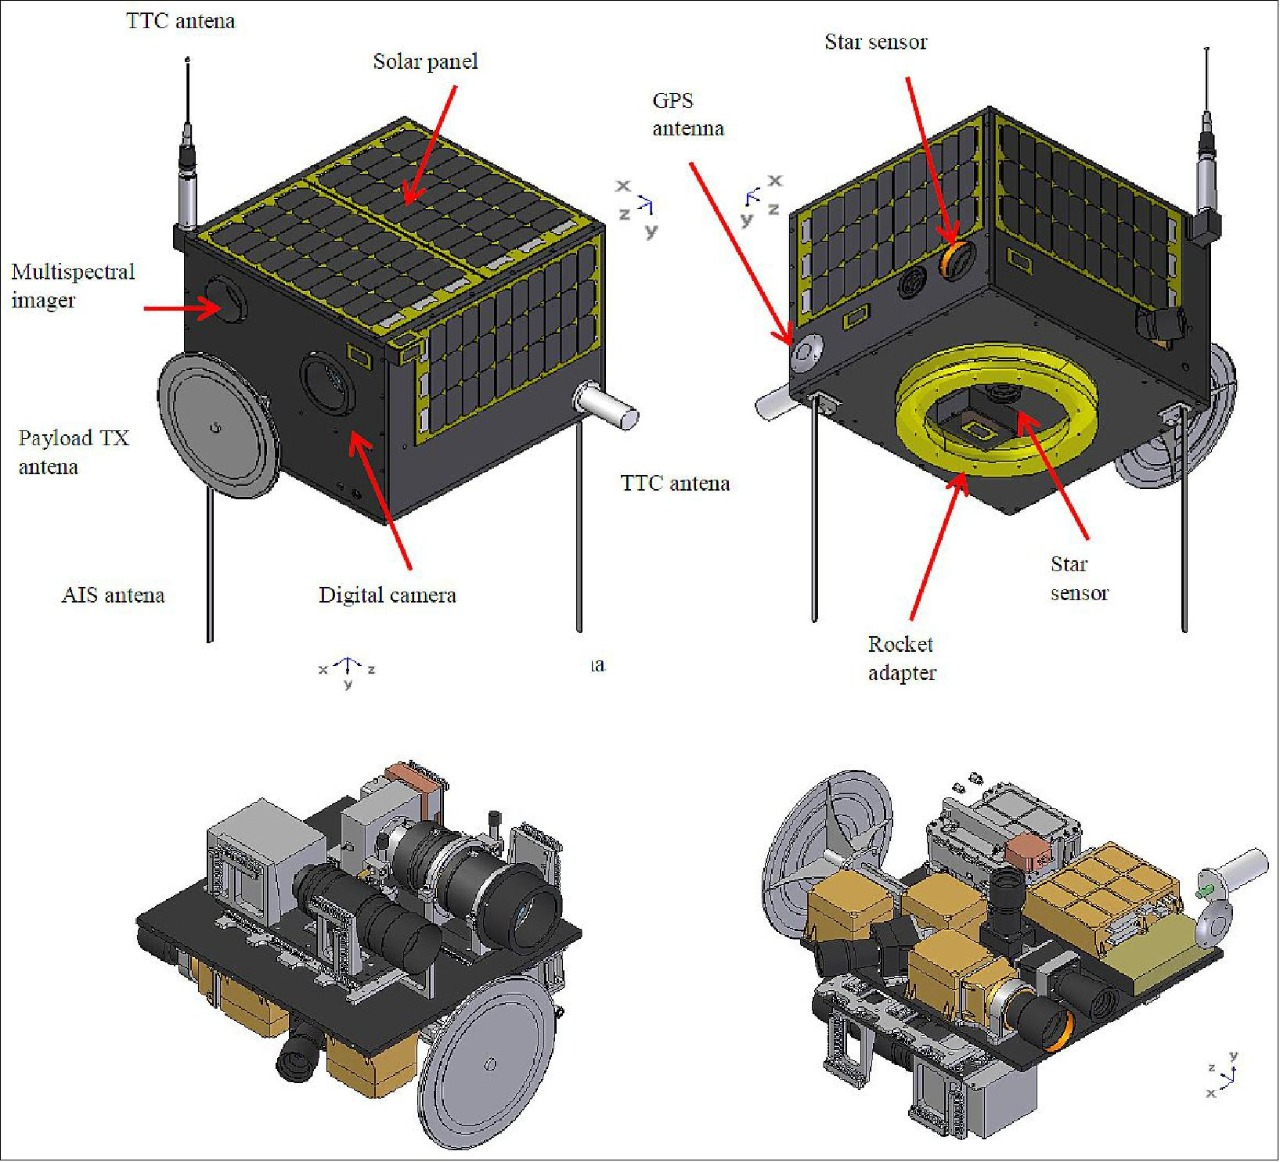
\includegraphics[width=0.7\textwidth]{fig/a3overview.jpg}
\caption{Desain LAPAN-A3}
\label{fig:a3overview}
\end{center}
\end{figure}

LAPAN-A3 memiliki misi utama untuk mendukung ketahanan pangan nasional melalui
pemantauan Bumi, khususnya di wilayah Indonesia. Untuk melakukan misi tersebut,
LAPAN-A3 dilengkapi 4 \textit{payload} utama \cite{hartono2019}. Pertama,
LAPAN-A3 dilengkapi dengan \textit{payload} utama berupa instrumen pencitra
multi-spekstral yang juga dikenal sebagai \textit{Line Imager Space
Application} (LISA). LISA terdiri dari sensor citra multi-spektral KLI-8023
yang dapat menangkap 4 spektrum cahaya (merah, hijau, biru, dan \textit{near
infra-red}) serta memiliki rentang suhu operasi minimum 0 \degree C dan
maksimum 70 \degree C \cite{semiconductor2017}. Hasil pengambilan citra Bumi
digunakan untuk memonitor penggunaan lahan, kondisi lingkungan, dan kesehatan
tanaman panen.

Selain LISA, LAPAN-A3 juga dilengkapi \textit{Digital Space Camera} (DSC) untuk
menglibrasi LISA serta mengobservasi lebih lanjut lokasi yang diinginkan serta
\textit{Automatic Identification System} (AIS) untuk memonitor lalu lintas
maritim. AIS dapat mengidentifikasi kapal yang melintas di perairan Indonesia
serta melacak kapal tersebut jika terjadi pelanggaran hukum maritim. Terakhir,
LAPAN-A3 juga membawa \textit{payload} pencitra termal eksperimental
\textit{micro-bolometer}.

Orbit LAPAN-A3 adalah orbit lingkaran \textit{sun-synchronous} dengan
ketinggian 515 km dan sudut inklinasi 97.5 \degree. Satelit dengan orbit
\textit{sun-synchronous} memiliki vektor normal orbit satelit yang membentuk
sudut konstan terhadap vektor arah Matahari-Bumi \cite{mortari}. Dengan begitu,
satelit tersebut akan mendapatkan pencahayaan yang cukup konsisten sepanjang
tahun dan akan melintasi khatulistiwa Bumi pada waktu lokal yang relatif sama
setiap harinya meski tetap membutuhkan maneuver koreksi secara berkala.

Karakteristik orbit \textit{sun-synchronous} LAPAN-A3 digunakan dalam
pengambilan citra Bumi lewat LISA untuk penyamaan kondisi pencahayaan saat
pengambilan citra antar observasi untuk seluruh wilayah cakupan observasi
LAPAN-A3. Dalam 1 hari, LAPAN-A3 biasanya dapat melakukan kontak dengan stasiun
kendali sebanyak 2 kali (siang dan malam) selama kurang lebih 11 menit. Orbit
LAPAN-A3 juga terus dijaga sehingga dapat mencakup wilayah Indonesia dan
memungkinkan pengunduhan data mendekati waktu \textit{real-time} dalam kondisi
\textit{downlink}. Gambar \ref{fig:coverage} menunjukkan cakupan wilayah
Indonesia dari hasil pengambilan citra oleh LAPAN-A3 sejak Januari 2017 sampai
dengan tahun 2018. 

\begin{figure}[H]
\setlength\belowcaptionskip{-0.7\baselineskip}
\begin{center}
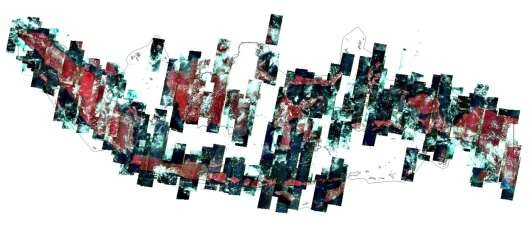
\includegraphics[width=0.5\textwidth]{fig/coverage.png}
	\caption{Cakupan wilayah Indonesia dari hasil pengambilan citra LAPAN-A3 \cite{hakim2018}}
\label{fig:coverage}
\end{center}
\end{figure}

Kebutuhan energi LAPAN-A3 dipenuhi dari tangkapan sinar Matahari oleh 5 panel
surya yang tersebar di 4 sisi satelit. Untuk mendeteksi arah sinar Matahari,
setiap sisi satelit LAPAN-A3 dilengkapi dengan \textit{coarse sun sensor}
(CSS). Gambar \ref{fig:css} menunjukkan contoh penempatan sensor Matahari pada
satelit. Jika sinar Matahari mengenai sensor pada permukaan sisi satelit, akan
muncul arus listrik yang proporsional dengan nilai cosinus sudut antara sinar
Matahari dan garis normal permukaan satelit $\theta_i$ sesuai persamaan berikut
\cite{zahran2009}:

\begin{equation}
\label{eq:current}
	\cos{\theta_i} = \frac{I_i}{I_0}
\end{equation}

dengan $I_i$ merupakan bacaan arus sensor Matahari \textit{node} dan $I_0$ arus
maksimum sensor Matahari satelit.

\begin{figure}[H]
\setlength\belowcaptionskip{-0.7\baselineskip}
\begin{center}
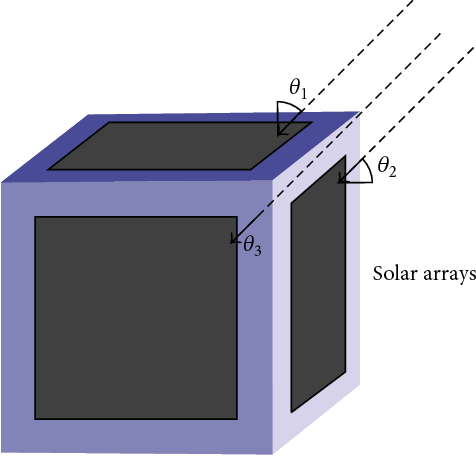
\includegraphics[width=0.5\textwidth]{fig/css.png}
	\caption{Contoh penempatan sensor Matahari pada satelit \cite{post2013}}
\label{fig:css}
\end{center}
\end{figure}

\section{Two-line Element}

Format data \textit{two-line element} atau TLE mendeskripsikan parameter orbit
objek ruang angkasa yang mengorbit Bumi pada suatu waktu tertentu. TLE dirilis
secara berkala ke publik oleh \textit{United States Space Command} (USSPACECOM)
yang melacak semua objek angkasa di orbit Bumi yang dapat dideteksi. Setiap
kolom dan baris TLE memiliki peruntukkan parameter tersendiri seperti yang
dapat dilihat pada Gambar \ref{fig:tlemeaning}. Secara singkat, TLE dapat
digunakan untuk menghitung vektor posisi dan kecepatan satelit yang mengorbit
Bumi dengan menggunakan algoritma bernama SGP4 yang telah diprogram pada kode
sumber TLE \cite{vallado2008}.

\begin{figure}[H]
\setlength\belowcaptionskip{-0.7\baselineskip}
\begin{center}
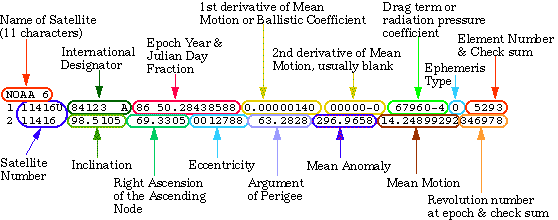
\includegraphics[width=0.5\textwidth]{fig/tlemeaning.png}
	\caption{Arti kolom dan baris TLE \cite{2011}}
\label{fig:tlemeaning}
\end{center}
\end{figure}

Algoritma SGP4 ditulis dalam bahasa pemrograman Fortran \cite{vallado2006},
tapi saat ini sudah diimplementasikan dalam banyak bahasa pemrograman lain
seperti Python. Pada karya tulis ini, TLE satelit LAPAN-A3 selama periode
observasi diambil dari situs Celestrak \cite{kelso}. TLE yang dikumpulkan
kemudian dijadikan acuan untuk propagasi orbit satelit LAPAN-A3 menggunakan
bahasa pemrograman Python lewat modul Skyfield.

\section{Pemodelan Termal Satelit}

Pemodelan termal satelit bertujuan untuk memodelkan karakteristik termal
satelit. Hal ini dapat dilakukan dengan menganalisis perpindahan panas yang
terjadi pada satelit sehingga didapatkan persamaan matematis yang
mendeskripsikan karakteristik termal satelit. Sebagai contoh, pemodelan termal
satelit dapat dilakukan dengan menghitung persamaan yang menggambarkan hubungan
perubahan suhu satelit seiring perubahan waktu. Pada karya tulis ini, pemodelan
termal satelit dilakukan secara semi-empiris. Hal ini berarti pemodelan termal
satelit dilakukan dengan menggunakan asumsi, pendekatan, dan generalisasi untuk
menyederhanakan perhitungan teoretis berdasarkan hasil observasi pada satelit.

Perpindahan panas yang terjadi pada satelit dapat dibagi menjadi perpindahan
panas secara internal dan eskternal. Perpindahan panas internal terjadi antar
komponen satelit lewat konduksi, konveksi, atau radiasi sedangkan perpindahan
panas eksternal umumnya terjadi antara satelit dan lingkungannya melalui
radiasi. Gambar \ref{fig:externalsource} menggambarkan sumber
perpidahan panas eksternal untuk satelit yang mengorbit Bumi.

\begin{figure}[H]
\setlength\belowcaptionskip{-0.7\baselineskip}
\begin{center}
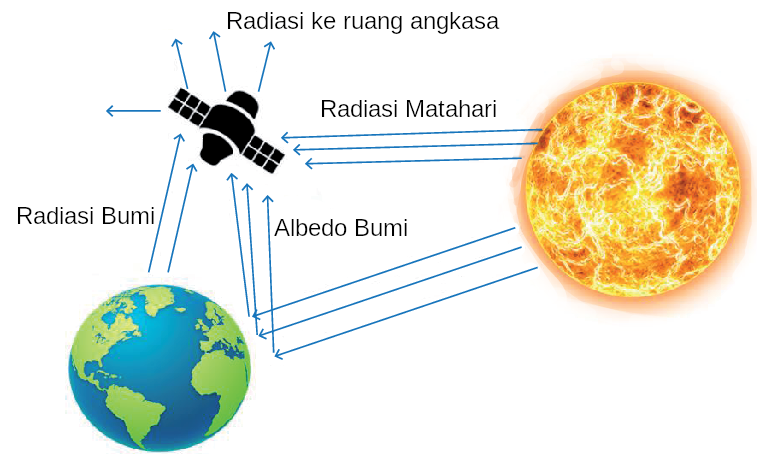
\includegraphics[width=0.5\textwidth]{fig/external_source.png}
	\caption{Sumber perpindahan panas eksternal satelit yang mengorbit Bumi \cite{abdelkhalek2019}}
\label{fig:externalsource}
\end{center}
\end{figure}

Pemodelan termal satelit biasanya dilakukan dengan membagi satelit menjadi
beberapa titik analisis diskrit atau \textit{node}. Setiap \textit{node}
mewakili bagian satelit yang dianggap memiliki karakteristik termal dan suhu
sama (isotermal). Pemodelan termal paling sederhana mengasumsikan satelit
sebagai 1 \textit{node} dengan suhu rata-rata satelit. Kemudian, dapat juga
dilakukan pemodelan dengan 2 \textit{node} : 1 \textit{node} untuk bagian luar
satelit dan 1 \textit{node} lainnya untuk bagian dalam satelit. Lalu, untuk
memodelkan karakteristik termal satelit secara lebih akurat, dapat digunakan
model \textit{node} banyak dengan jumlah yang disesuaikan dengan kebutuhan
pemodelan. Pendekatan model \textit{node} banyak ini akan digunakan pada karya
tulis ini

Untuk sebuah model termal umum satelit dengan N \textit{node} yang mengorbit
Bumi, persamaan keseimbangan termal
sebuah \textit{node} $i$ yang sudah memperhitungkan sumber masukan dan keluaran
panas serta interaksi dengan \textit{node-node} lain $j$ dapat dituliskan
sebagai berikut \cite{martinez2022}:

\begin{equation}
\label{eq:qeq}
\begin{split}
	C_{i} \frac{\Delta T_i}{\Delta t} = &\ \dot{Q}_{S,i}(t)\\
	&+ \dot{Q}_{a,i}(t) \\
	&+ \dot{Q}_{E,i}(t) \\
	&- \dot{Q}_{\infty,i}(t) \\
	&+ \mathop{\sum_{j=1}^{N}}_{j \neq i} \dot{Q}_{cond,ij}(t) \\
	&+ \mathop{\sum_{j=1}^{N}}_{j \neq i} \dot{Q}_{rad,ij}(t) \\
	&+ \dot{Q}_{dis,i}
\end{split}
\end{equation}

dengan $C_i$ kapasitas termal rata-rata \textit{node}, $\Delta T_i$ perubahan
suhu \textit{node}, $\Delta t$ selang waktu, $T_i$ suhu \textit{node}, $T_j$
suhu \textit{node-node} lain, $\dot{Q}_{S,i}$ laju masukan panas akibat radiasi dari
Matahari, $\dot{Q}_{a,i}$ laju masukan panas akibat albedo Bumi,
$\dot{Q}_{E,i}$ laju masukan panas akibat radiasi dari Bumi, $\dot{Q}_{\infty,i}$
laju keluaran panas akibat disipasi ke lingkungan ruang angkasa,
$\dot{Q}_{cond,ij}$ laju masukan panas ke \textit{node i} akibat konduksi dari \textit{node j},
$\dot{Q}_{rad,ij}$ laju masukan panas ke \textit{node i} akibat radiasi dari
\textit{node j}, dan  $\dot{Q}_{dis,i}$ laju masukan panas akibat disipasi
elektrik \textit{node}.

Persamaan \ref{eq:qeq} mengasumsikan satelit memiliki sistem kendali termal
pasif sehingga memiliki nilai $\dot{Q}_{dis,i}$ konstan terhadap waktu serta
perpindahan panas antar \textit{node} satelit terjadi akibat konduksi dan
radiasi saja. Selain itu, suhu lingkungan ruang angkasa (2.7 K) dianggap jauh
lebih kecil daripada rentang suhu yang mungkin dicapai satelit. Penjabaran
suku-suku termal pada Persamaan \ref{eq:qeq} menghasilkan Persamaan
\ref{eq:raweq}:

\begin{equation}
\label{eq:raweq}
\begin{split}
	C_{i} \frac{\Delta T_i}{\Delta t} = &\ \left(\alpha_{s,i} - \eta F_{pg,i}\right) E_s A_i \cos{\theta_{i}(t)} F_{e,i}(t) \\
	&+ \left(\alpha_{s,i} - \eta F_{pg,i}\right)\rho_{E} E_s A_i F_{i,E}(t) \cos{\beta} F_a(t) \\
	&+ \varepsilon_i A_i F_{i,E}(t) \varepsilon_E \sigma T_{i}(t)^4 \\
	&- \varepsilon_i A_i F_{i,\infty}(t) \sigma T_{i}(t)^4 \\
	&+ \mathop{\sum_{j=1}^{N}}_{j \neq i} G_{ij} \left(T_j(t) - T_i(t)\right) \\
	&+ \mathop{\sum_{j=1}^{N}}_{j \neq i} \sigma R_{ij}(T_{j}(t)^4-T_{i}(t)^4) \\
	&+ \dot{Q}_{dis,i}
\end{split}
\end{equation}

dengan $T_i$ suhu \textit{node}, $T_j$ suhu \textit{node-node} lain,
$\alpha_{s,i}$ absorpsi surya total \textit{node}, $\eta$ efisiensi listrik panel surya,
$F_{pg,i}$ rasio luas panel surya terhadap luas \textit{node}, $E_s$ penyinaran surya
tegak lurus terhadap arah Matahari, $A_i$ luas \textit{node}, $\theta_i$ sudut antara
garis normal permukaan \textit{node} dengan sinar Matahari, $F_{e,i}$ faktor gerhana
\textit{node}, $\rho_E$ albedo Bumi, $F_{i,E}$ \textit{view factor} \textit{node} ke Bumi, $\beta$ sudut
antara bidang orbit satelit dengan vektor Matahari, $F_a$ faktor albedo
satelit, $\varepsilon_i$ emisivitas \textit{node}, $\varepsilon_E$ emisivitas Bumi, $\sigma$
konstanta Stefan–Boltzmann, $F_{i,\infty}$ \textit{view factor} \textit{node} terhadap
lingkungan ruang angkasa, $G_{ij}$ koefisien kopling konduksi antara \textit{node} $i$
dan $j$, serta $R_{ij}$ koefisien kopling radiasi antara \textit{node} $i$ dan $j$.

\section{Persamaan Termal Satelit LAPAN-A3}

Pendekatan analisis termal konvensional mengharuskan perhitungan semua variabel
suku di ruas kanan Persamaan \ref{eq:raweq} untuk mendapatkan persamaan termal
yang dapat mendeskripsikan karakteristik termal satelit. Karena pendekatan yang
digunakan untuk memodelkan LAPAN-A3 secara termal adalah regresi linear lewat
metode \textit{machine learning}, Persaman \ref{eq:raweq} harus diubah menjadi
bentuk linear terlebih dahulu. Lebih spesifik lagi, persamaan termal yang akan
dihitung untuk LAPAN-A3 adalah persamaan laju perubahan suhu \textit{node}
satelit.

LAPAN-A3 merupakakan satelit mengorbit Bumi secara \textit{sun-synchronous}
sehingga memiliki orientasi terhadap Matahari yang sama sepanjang tahun serta
kondisi pencahayaan yang cukup konsisten juga. Dengan demikian, nilai
\textit{view factor} \textit{node} LAPAN-A3 ke lingkungan $F_{i,\infty}$
dianggap konstan. Satelit LAPAN-A3 juga dilengkapi sensor sinar Matahari pada
setiap sisinya sehingga sudut antara garis normal permukan \textit{node} dengan
sinar Matahari dapat dihitung berdasarkan Persamaan \ref{eq:current} yang sudah
dijabarkan sebelumnya.

Selanjutnya, untuk memudahkan penulisan dan penurunan persamaan,
variabel-variabel pada 4 suku pertama Persamaan \ref{eq:raweq} yang tidak
berubah terhadap waktu selama periode observasi dapat digantikan dengan
koefisien-koefisien sesuai persamaan berikut :

\begin{equation}
\label{eq:short}
\begin{split}
	c_{S} &= \left(\alpha_{s,i} - \eta F_{pg,i}\right) E_s A_i \\
	c_{a} &= \left(\alpha_{s,i} - \eta F_{pg,i}\right)\rho_{E} E_s A_i \cos{\beta} \\
	c_{E} &= \varepsilon_i A_i \varepsilon_E \\
	c_{env} &= \varepsilon_i A_i F_{i,\infty} \sigma
\end{split}
\end{equation}

dengan $c_{S}$ merupakan koefisien suku panas akibat Matahari, $c_{a}$
koefisien suku panas akibat albedo, $c_{E}$ koefisien suku panas akibat Bumi,
dan $c_{env}$ koefisien suku disipasi ke lingkungan ruang angkasa.

Lewat substitusi nilai $\cos{\theta_i}$ dengan Persamaan \ref{eq:current} serta
koefisien-koefisien pada Persamaan \ref{eq:short} dan pembagian kedua ruas
persamaan dengan $C_i$ disertai perubahan urutan suku-suku,
Persamaan \ref{eq:raweq} dapat dijadikan persamaan linear variabel banyak
dengan ketentuan sebagai berikut :

\begin{itemize}
	\item Laju perubahan suhu \textit{node} $\frac{\Delta T_i}{\Delta t}$ sebagai variabel dependen
	\item Variabel yang berubah terhadap waktu (ditandai dengan $(t)$ pada Persamaan \ref{eq:raweq}) sebagai variabel independen
	\item Variabel yang tetap terhadap waktu sebagai gradien
	\item Konstanta suku disipasi energi $\frac{\dot{Q}_{dis,i}}{C_i}$ sebagai titik potong (\textit{intercept})
\end{itemize}

Dengan demikian, didapatkan persamaan laju perubahan suhu \textit{node} LAPAN-A3 sebagai berikut :

\begin{equation}
\label{eq:lineq}
\begin{split}
	\frac{\Delta T_i}{\Delta t} = &\ \frac{c_S}{C_i I_0} I_{i}(t) F_{e,i}(t) \\
	&+ \frac{c_a}{C_i} F_{i,E}(t) F_a(t) \\
	&+ \frac{c_E}{C_i} F_{i,E}(t) T_{i}(t)^4 \\
	&- \frac{\left( \mathop{\sum_{j=1}^{N}}_{j \neq i} \sigma R_{ij} + c_{env} \right) }{C_i} T_{i}(t)^4 \\
	&+ \mathop{\sum_{j=1}^{N}}_{j \neq i} \frac{G_{ij}}{C_i} \left(T_j(t) - T_i(t)\right) \\
	&+ \mathop{\sum_{j=1}^{N}}_{j \neq i} \frac{\sigma R_{ij}}{C_i}T_{j}(t)^4 \\
	&+ \frac{\dot{Q}_{dis,i}}{C_i}
\end{split}
\end{equation}

Persamaan \ref{eq:lineq} merupakan persamaan linear variabel banyak biasa yang
dapat diselesaikan lewat regresi linear serta akan digunakan dalam model
\textit{machine learning} karya tulis ini. Dapat dilihat juga dari Persamaan
\ref{eq:lineq} bahwa jumlah variabel yang harus dihitung telah berkurang
menjadi hanya variabel yang berubah terhadap waktu atau hasil perkaliannya
karena model regresi linear dapat menghitung koefisien dan konstanta persamaan
yang tersisa. Selain itu, variabel seperti suhu \textit{node-node} satelit
dapat langsung diketahui dari data telemetri satelit LAPAN-A3 sehingga praktis
variabel yang perlu dihitung hanya 3 faktor panas satelit. Secara singkat,
Tabel \ref{table:unknown} merangkum variabel yang masih perlu diketahui.

\begin{table}[!ht]
\begin{center}
\caption{Variabel yang masih perlu diketahui}
\label{table:unknown}
\begin{tabular}{|l|l|}
\hline
Variabel & Deskripsi \\ \hline
	$I_i F_{e,i}$        & Faktor panas akibat Matahari         \\ \hline
	$F_{i,E} F_a$        & Faktor panas akibat albedo         \\ \hline
	$F_{i,E} T_i^4$        & Faktor panas akibat Bumi         \\ \hline
	$T_i, T_j, T_i^4,$ dan $T_j^4$        & Suhu \textit{node-node} satelit         \\ \hline
\end{tabular}
\end{center}
\vspace{-5mm}
\end{table}

\section{Perhitungan Faktor Gerhana Node Satelit}

Faktor gerhana \textit{node} satelit $F_{e,i}$ diperlukan untuk menghitung faktor panas
akibat Matahari. Secara singkat, parameter ini akan bernilai 1 jika \textit{node}
menerima sinar Matahari dan sebaliknya bernilai 0 jika \textit{node} dalam fase gerhana
(tidak menerima sinar Matahari).

\section{Perhitungan View Factor Node Satelit ke Bumi}

Dalam perpindahan panas akibat radiasi, \textit{view factor} merupakan proporsi
radiasi dari suatu permukaan yang diterima oleh permukaan lain. Dengan
demikian, \textit{view factor} dari \textit{node} satelit ke Bumi merupakan
proporsi radiasi panas yang diterima permukaan Bumi dari permukaan
\textit{node} satelit. Nilai \textit{view factor} antara 2 permukaan murni
bergantung dari bentuk atau geometri kedua permukaan tersebut.

Secara umum, untuk sebuah permukaan 1 yang memancarkan radiasi ke permukaan 2 seperti yang
ditampilkan pada Gambar \ref{fig:viewfactor}, \textit{view factor} dari
permukaan 1 ke 2 $F_{1,2}$ dapat ditentukan lewat persamaan berikut
\cite{muneer2020}:

\begin{equation}
\label{eq:viewfactor}
	F_{1,2} = \frac{1}{A_1} \int_{A_1} \int_{A_2} \frac{\cos{\Phi_1} \cos{\Phi_2}}{\pi R_{12}} dA_2 dA_1
\end{equation}

dengan $A_1$ merupakan luas permukaan 1, $A_2$ luas permukaan 2, $dA_1$ elemen
diferensial permukaan 1, $dA_2$ elemen diferensial permukaan 2, $R_{12}$ jarak
antara $dA_1$ dan $dA_2$, dan $\Phi_1$ serta $\Phi_2$ sudut antara vektor
normal masing-masing elemen diferensial permukaan dengan garis $R$.  

\begin{figure}[!ht]
\setlength\belowcaptionskip{-0.7\baselineskip}
\begin{center}
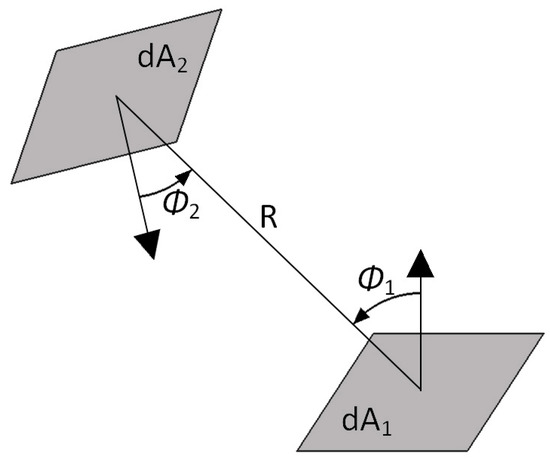
\includegraphics[width=0.5\textwidth]{fig/viewfactor.jpg}
	\caption{Ilustrasi geometri perhitungan \textit{view factor} \cite{muneer2020}}
\label{fig:viewfactor}
\end{center}
\end{figure}

Solusi analitik Persamaan \ref{eq:viewfactor} hanya tersedia
untuk kasus bentuk permukaan sederhana seperti plat, bola, dan tabung.
Untuk bentuk permukaan yang lebih kompleks, Persamaan
\ref{eq:viewfactor} harus diselesaikan secara numerik semisal
menggunakan metode Monte-Carlo, perangkat lunak komersial yang memang
dirancang untuk menghitung \textit{view factor} geometri kompleks,
atau metode numerik lainnya.

Dari bagian Batasan Penelitian, satelit LAPAN-A3 diasumsikan berbentuk
balok. Dengan demikian, \textit{node} yang mewakili sisi-sisi
satelit dapat dianggap berbentuk plat persegi panjang. Selanjutnya, ukuran
satelit jauh lebih kecil dari Bumi sehingga sisi satelit dapat didekati dengan
elemen diferensial plat persegi panjang terhadap Bumi. Dengan begitu, nilai
\textit{view factor} \textit{node} satelit ke Bumi dapat didekati
dengan perhitungan analitik bentuk dasar plat persegi panjang
(\textit{node}) ke bola (Bumi). 

Semisal, akan dicari nilai \textit{view factor} dari permukaan plat persegi
panjang ke permukaan bola dengan jari-jari $r$ seperti yang ditampilkan pada
Gambar \ref{fig:platball}. Variabel $\gamma$ merupakan sudut antara vektor
normal permukaan plat $\hat{n}$ dengan garis jarak antara kedua permukaan $H$.

\begin{figure}[!ht]
\setlength\belowcaptionskip{-0.7\baselineskip}
\begin{center}
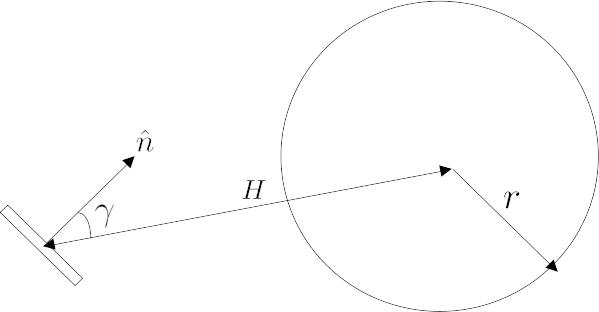
\includegraphics[width=0.5\textwidth]{fig/platball.png}
	\caption{Ilustrasi \textit{view factor} dari plat ke bola}
\label{fig:platball}
\end{center}
\end{figure}

Untuk mempermudah perhitungan \textit{view factor}, akan didefinisikan 3 variabel sebagai berikut :

\begin{equation}
\begin{split}
\label{eq:hxy}
	h &\equiv \frac{H}{r} \\
	x &\equiv \sqrt{h^2 - 1} \\
	y &\equiv -x \cot{\gamma}
\end{split}
\end{equation}

Nilai \textit{view factor} dari permukaan plat persegi panjang 1 ke permukaan
bola 2 kemudian dapat dihitung berdasarkan persamaan berikut \cite{martinez2022a}:

\begin{equation}
	F_{1,2} = 
\begin{cases} 
	\frac{\cos{\gamma}}{h^2} & ,\;|\gamma| \leq \cos^{-1}\left(\frac{1}{h}\right) \\
	\frac{1}{\pi h^2} \left( \cos{\gamma}\cos^{-1}y - x\sin{\gamma}\sqrt{1-y^2} \right) + \frac{1}{\pi}\tan^{-1}\left( \frac{\sin{\gamma}\sqrt{1-y^2}}{x} \right) & ,\;|\gamma| > \cos^{-1}\left(\frac{1}{h}\right) \\
\end{cases}
\label{eq:vf}
\end{equation}

\section{Perhitungan Faktor Albedo Satelit}

Masukan panas dari albedo pada satelit bersumber dari radiasi sinar Matahari
yang dipantulkan benda langit seperti planet, bulan, atau wahana antariksa
lain. Pada LAPAN-A3, albedo yang diterima satelit berasal dari sinar Matahari
yang dipantulkan oleh Bumi. Karena itu, faktor albedo LAPAN-A3 mewakili
proporsi radiasi pantulan yang diterima satelit dari Bumi. Faktor albedo
satelit bernilai 0 saat satelit memasuki fase gerhana dan bernilai 1 saat
satelit berada pada titik \textit{subsolar}, titik di orbit satelit yang
memiliki jarak paling dekat dengan Matahari. 

Secara umum, faktor albedo satelit dapat dituliskan sebagai berikut :

\begin{equation}
\label{eq:albedofactor}
F_a = \left( \frac{1 + \cos{\phi}}{2} \right)^2 \left[ 1 - \left( \frac{\phi}{\phi_{es}} \right)^2 \right] F_e
\end{equation}

dengan $\phi$ merupakan posisi sudut satelit, $\phi_{es}$ posisi sudut satelit
saat memasuki fase gerhana, dan $F_e$ faktor gerhana satelit. Kedua posisi
sudut dihitung dari titik \textit{subsolar}. Faktor gerhana satelit sendiri
bernilai 0 jika satelit dalam fase gerhana dan sebaliknya bernilai 1 jika
satelit tidak dalam fase gerhana.

\section{Machine Learning}

Bidang \textit{machine learning} secara umum mempelajari metode dan algoritma
komputer yang dapat menggunakan data untuk meningkatkan performa dalam
mengerjakan serangkaian tugas secara otomatis \cite{mitchell1997}. Bidang ini
termasuk dalam bagian dari kecerdasan buatan (\textit{artificial intelligence})
dan aplikasinya memungkinkan komputer untuk mengenali pola dalam data sehingga
dapat memperoleh pengetahuan dari data tersebut tanpa pemrograman eksplisit
\cite{v2020}. Gambar \ref{fig:aiml} menunjukkan posisi \textit{machine learning}
sebagai bagian dari kecerdasan buatan.

\begin{figure}[H]
\setlength\belowcaptionskip{-0.7\baselineskip}
\begin{center}
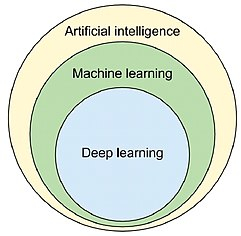
\includegraphics[width=0.3\textwidth]{fig/aiml.jpg}
	\caption{Bidang \textit{machine learning} sebagai bagian dari kecerdasan buatan \cite{2020}}
\label{fig:aiml}
\end{center}
\end{figure}

Algoritma \textit{machine learning} mampu mempelajari sendiri karakteristik
permasalahan yang perlu diselesaikan dari kumpulan data yang diberikan tanpa
intervensi operator manusia. Karena itu, metode \textit{machine learning} sudah
umum digunakan dalam penyelesaian berbagai permasalahan dalam bidang-bidang
lain. Sebagai contoh, pengelompokan wajah manusia, pembuatan rekomendasi
produk, dan analisis finansial modern lazim menggunakan metode \textit{machine
learning}. Implementasi algoritma pembuatan \textit{machine learning} sudah
dilakukan untuk berbagai bahasa pemrograman termasuk bahasa pemrograman Python.

Gambar \ref{fig:mldiagram} menunjukkan diagram cara kerja metode
\textit{machine learning} secara umum untuk menyelesaikan suatu masalah.
Dataset latihan berupa kumpulan data yang akan dianalisis diberikan kepada
algoritma \textit{machine learning}. Dari dataset latihan tersebut, algoritma
\textit{machine learning} akan membuat hipotesis berupa model yang
mendeskripsikan pola-pola dan hubungan antar elemen data masukan. Hipotesis
model kemudian diterapkan ke data pengujian dan hasil evaluasi performa
keluaran dari data pengujian tersebut dijadikan umpan balik untuk meningkatkan
performa iterasi model selanjutnya.

\begin{figure}[H]
\setlength\belowcaptionskip{-0.7\baselineskip}
\begin{center}
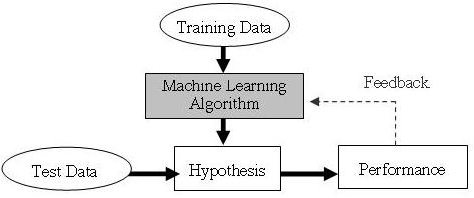
\includegraphics[width=0.5\textwidth]{fig/mldiagram.jpg}
	\caption{Cara kerja metode \textit{machine learning} secara umum \cite{2012}}
\label{fig:mldiagram}
\end{center}
\end{figure}

Metode \textit{machine learning} secara umum dapat terbagi menjadi 3 kategori
luas : \textit{supervised learning}, \textit{unsupervised learning}, dan
\textit{reinforcement learning} \cite{russell1995}. Metode \textit{supervised learning} dilakukan
dengan memberikan komputer dataset yang sudah dilabeli berupa data masukan dan
data keluaran yang diinginkan. Algoritma \textit{machine learning} kemudian
akan mencoba membuat hubungan matematis yang memetakan data masukan ke data
keluaran. Sebagai contoh, model \textit{machine learning} untuk mengkategorikan
bunga dapat diberikan data masukan gambar bunga dan data keluaran jenis bunga.

Selanjutnya, metode \textit{unsupervised learning} menggunakan data masukan
yang tidak dilabeli sehingga algoritma \textit{machine learning} harus
menentukan sendiri struktur dari data masukan tersebut. Metode ini dapat
digunakan menemukan pola dan fitur dari data masukan. Terakhir, pada metode
\textit{reinforcement learning} komputer akan diberikan suatu tujuan dan
dibiarkan berinteraksi dengan sistem yang akan memberikan umpan balik berupa
\textit{reward} dan \textit{penalty}. Model \textit{reinforcement learning}
akan berusaha mencari rangkaian tindakan untuk mencapai tujuan yang dapat
memaksimalkan \textit{reward} dan meminimalkan \textit{penalty}.

\subsection{Aplikasi Machine Learning Dalam Pemodelan Termal Satelit}

Aplikasi metode \textit{machine learning} dalam analisis termal secara umum
dapat dibagi menjadi 2 : inferensi dan prediksi. Inferensi merupakan proses
pembuatan model matematis yang menggambarkan hubungan variabel-variabel dalam
cara kerja suatu sistem sedangkan prediksi adalah proses pembuatan prakiraan
hasil masa depan atau variabel yang belum diobservasi berdasarkan data
observasi yang sudah ada. Dalam konteks pemodelan termal satelit, inferensi
dapat digunakan untuk menghitung kontribusi tiap suku dalam persamaan termal
satelit sehingga dampak masing-masing suku secara individual dapat diketahui.
Prediksi sendiri dapat digunakan untuk menentukan besaran parameter termal yang
sebelumnya tidak diketahui berdasarkan parameter yang sudah diketahui.

Dalam karya tulis ini, prediksi menggunakan metode \textit{machine learning}
akan digunakan untuk menyelesaikan persamaan laju perubahan suhu \textit{node}
satelit seperti yang dituliskan pada Persamaan \ref{eq:lineq}. Secara spesifik,
metode \textit{machine learning} yang digunakan adalah pemodelan regresi linear
menggunakan bahasa pemrograman Python yang dilatih menggunakan data TLE beserta
data telemetri satelit LAPAN-A3 untuk periode observasi 19 dan 20 Mei 2018.

Regresi linear merupakan pendekatan untuk memodelkan hubungan antara variabel
dependen dengan variabel independen secara linear. Lewat regresi linear,
hubungan antar variabel dependen dan variabel independen didekati lewat
persamaan linear umum sebagai berikut \cite{freedman2009}:

\begin{equation}
\label{eq:reglinear}
Y = Xw + \varepsilon
\end{equation}

dengan $Y$ adalah matriks variabel dependen, $X$ matriks variabel independen,
$w$ matriks koefisien yang tidak diketahui, serta
$\varepsilon$ matriks kesalahan atau gangguan. Pada model termal satelit
LAPAN-A3 yang ditampilkan pada Persamaan \ref{eq:lineq}, $Y$ mewakili laju
perubahan suhu \textit{node-node} satelit, $X$ parameter dan hasil perkalian parameter satelit yang
berubah terhadap waktu, $w$ koefisien suku-suku pada persamaan termal, dan
$\varepsilon$ kesalahan pada hasil pengukuran parameter.  

Model regresi linear \textit{machine learning} akan menghitung koefisien
suku-suku pada Persamaan \ref{eq:lineq} yang belum diketahui berdasarkan data
masukan model \textit{machine learning}. Hasil perhitungan koefisien suku-suku
pada persamaan termal tersebut kemudian akan digunakan untuk memprediksi laju
perubahan suhu \textit{node} dataset ujian model. Lewat prediksi laju perubahan
suhu \textit{node}, perubahan suhu \textit{node} dan suhu \textit{node} pada
selang waktu pengamatan berikutnya dapat diprediksi juga.

\subsection{Evaluasi Performa Model Machine Learning}

Untuk mengevaluasi performa prediksi regresi linear model \textit{machine
learning}, dapat digunakan skor koefisien determinasi ($R^2$) \cite{gupta2021}
dan nilai \textit{root mean squared error} (RMSE) \cite{zheng}. Perhitungan
skor $R^2$ dan nilai RMSE sesuai konteks model \textit{machine learning} sudah
tersedia pada modul \textit{machine learning} dalam bahasa pemrograman Python
yang dipakai dalam karya tulis ini sehingga sub-bagian ini hanya akan
mendeskripsikan kedua parameter tersebut.

Skor koefisien determinasi atau $R^2$ mengukur seberapa baik model regresi
memprediksi tren data observasi. Parameter ini bernilai maksimum 1 dan semakin
tinggi skor $R^2$, semakin dekat tren hasil prediksi model dengan tren data
observasi. Skor ini juga mengukur proporsi varians dalam data observasi yang
dapat dijelaskan oleh hasil prediksi model. Sebagai contoh, jika hasil prediksi
model regresi memiliki skor $R^2$ senilai 0.9, 90\% varians dalam data
observasi dapat dijelaskan oleh hasil prediksi model.

Nilai \textit{root mean squared error} atau RMSE mengukur seberapa besar
perbedaan antara hasil prediksi model dengan data observasi. RMSE selalu
bernilai positif dan semakin rendah nilai RMSE, semakin dekat pula prediksi
model regresi dengan data observasi. Parameter ini bergantung pada skala data
serta dataset yang digunakan oleh model. Karena itu, parameter ini dapat
dijadikan pembanding akurasi antara model-model yang memiliki dataset masukan
yang sama.

\section{Perangkat Lunak}

\subsection{Python}

Python adalah bahasa pemrograman umum yang diciptakan oleh Guido van
Rossum. Python umum digunakan untuk menyelesaikan permasalahan sains
data. Bahasa ini dipilih untuk melakukan perhitungan dan
pemodelan dalam karya tulis ini karena memiliki modul pemrograman yang
cukup lengkap, tidak terikat biaya lisensi, dan kode sumber-nya dapat
diakses secara publik. Versi bahasa Python yang digunakan pada karya
tulis ini adalah 3.10.

\subsection{Pandas}

Pandas adalah modul pemrogaman untuk bahasa Python yang diciptakan oleh Wes
McKinney. Modul ini biasa digunakan untuk mengolah dan menganalisis objek data
seperti baris dan kolom tabel \cite{reback2022}. Pada karya tulis ini, modul Pandas
digunakan untuk mengolah sumber data mentah berupa data telemetri satelit LAPAN
A3 agar dapat diproses lebih lanjut pada tahap pembuatan model termal satelit.

\subsection{Numpy}

Numpy adalah sebuah modul Python yang diciptakan oleh Travis Oliphant. Modul
ini digunakan untuk melakukan operasi pada matriks multi-dimensional secara
cepat dan efisien \cite{harris2020}. Karya tulis ini menggunakan Numpy untuk
menghitung dan menyimpan variabel-variabel yang dibutuhkan model termal satelit
seperti matriks sudut Euler satelit, matriks posisi satelit, dan lain-lain. 

\subsection{Matplotlib}

Matplotlib adalah modul Python untuk membuat plot dan grafik 2D \cite{hunter2007}.
Modul ini diciptakan oleh John Hunter dan umum digunakan pada proyek sains data
sebagai sarana visualisasi data. Karya tulis ini menggunakan modul Matplotlib
untuk menggambarkan hasil pemodelan termal satelit.

\subsection{Scikit-learn}

Scikit-learn merupakan modul pengolahan data, pembuatan model, validasi, dan
pengukuran performa model \textit{machine learning} dalam bahasa Python \cite{pedregosa2011}.
Modul ini pertama kali dikembangkan oleh David Cournapeau pada 2007 dan
mencakup algoritma-algoritma \textit{machine learning} untuk skala menengah.
Scikit-learn digunakan untuk pembuatan model \textit{machine learning} pada karya tulis
ini.

\subsection{Skyfield}

Skyfield adalah sebuah modul astronomi untuk perhitungan posisi bintang,
planet, dan satelit yang mengorbit di sekitar Bumi \cite{rhodes2019}. Modul ini
ditulis oleh Brandon Rhodes dan menggunakan implementasi algoritma SGP4 dalam
bahasa Python \cite{rodriguez} untuk memprediksi dinamika orbit satelit mengacu
format TLE. Karya tulis ini menggunakan Skyfield untuk
mensimulasikan orbit LAPAN-A3 selama periode observasi.

\subsection{Scipy}

Scipy adalah sebuah modul perhitungan saintifik dalam bahasa Python yang
dikembangkan pertama kali oleh Travis Oliphant, Pearu Peterson, dan Eric Jones
\cite{virtanen2020}. Modul ini memuat formula perhitungan aljabar, persamaan
diferensial, statistik, dan formula-formula umum lain. Pada karya tulis ini,
Scipy digunakan untuk menghitung skor standar data suhu \textit{node} satelit
untuk mendeteksi data \textit{outlier}.
